% \PassOptionsToPackage{showrules}{blurb}
% \PassOptionsToPackage{showframe}{blurb}
\documentclass[fleqn]{thesis}

% DOCUMENT
\usepackage{kantlipsum}

\graphicspath{{./ch3_creteil/img/}{./ch2_gridshell/img/}}

\def\dolist{\afterassignment\dodolist\let\next= }
\def\dodolist{\ifx\next\endlist \let\next\relax
   \else \\\let\next\dolist \fi
   \next}
\def\endlist{\endlist}
\def\hidehrule#1#2{\kern-#1%
   \hrule height#1 depth#2 \kern-#2 }
\def\hidevrule#1#2{\kern-#1{\dimen0=#1
     \advance\dimen0 by#2\vrule width\dimen0}\kern-#2 }
\def\makeblankbox#1#2{\hbox{\lower\dp0\vbox{\hidehrule{#1}{#2}%
     \kern-#1 % overlap the rules at the corners
     \hbox to \wd0{\hidevrule{#1}{#2}%
       \raise\ht0\vbox to #1{}% set the vrule height
       \lower\dp0\vtop to #1{}% set the vrule depth
       \hfil\hidevrule{#2}{#1}}%
     \kern-#1\hidehrule{#2}{#1}}}}
\def\maketypebox{\makeblankbox{0pt}{1pt}}
\def\makelightbox{\makeblankbox{.2pt}{.2pt}}
\def\\{\if\space\next\ % assume that \next is unexpandable
  \else \setbox0=\hbox{\next}\maketypebox\fi}
\def\demobox#1{\setbox0=\hbox{\dolist#1\endlist}%
   \leavevmode\copy0\kern-\wd0\makelightbox}

\begin{document}

\listoffigures

	\part{My First Part}
		\chapter{Mon premier chapitre}
		\section{Une section}
		\kant[1-4]
		\section{Une deuxième section}
		\kant[1-2]
		\section{Une troisième section}
		\kant[1-2]
	
	\part{My Second Part}
		% \chapter{Mon premier chapitre}
		% \section{Une section}
		% \kant[1-20]
		% \section{Une deuxième section}
		% \kant[1-2]
		% \section{Une troisième section}
		% \kant[1-2]
		\cref{fig:twospread}





	\clearpage
	% \begin{textblock*}{0.5\paperwidth}(0cm,0cm)
	% 	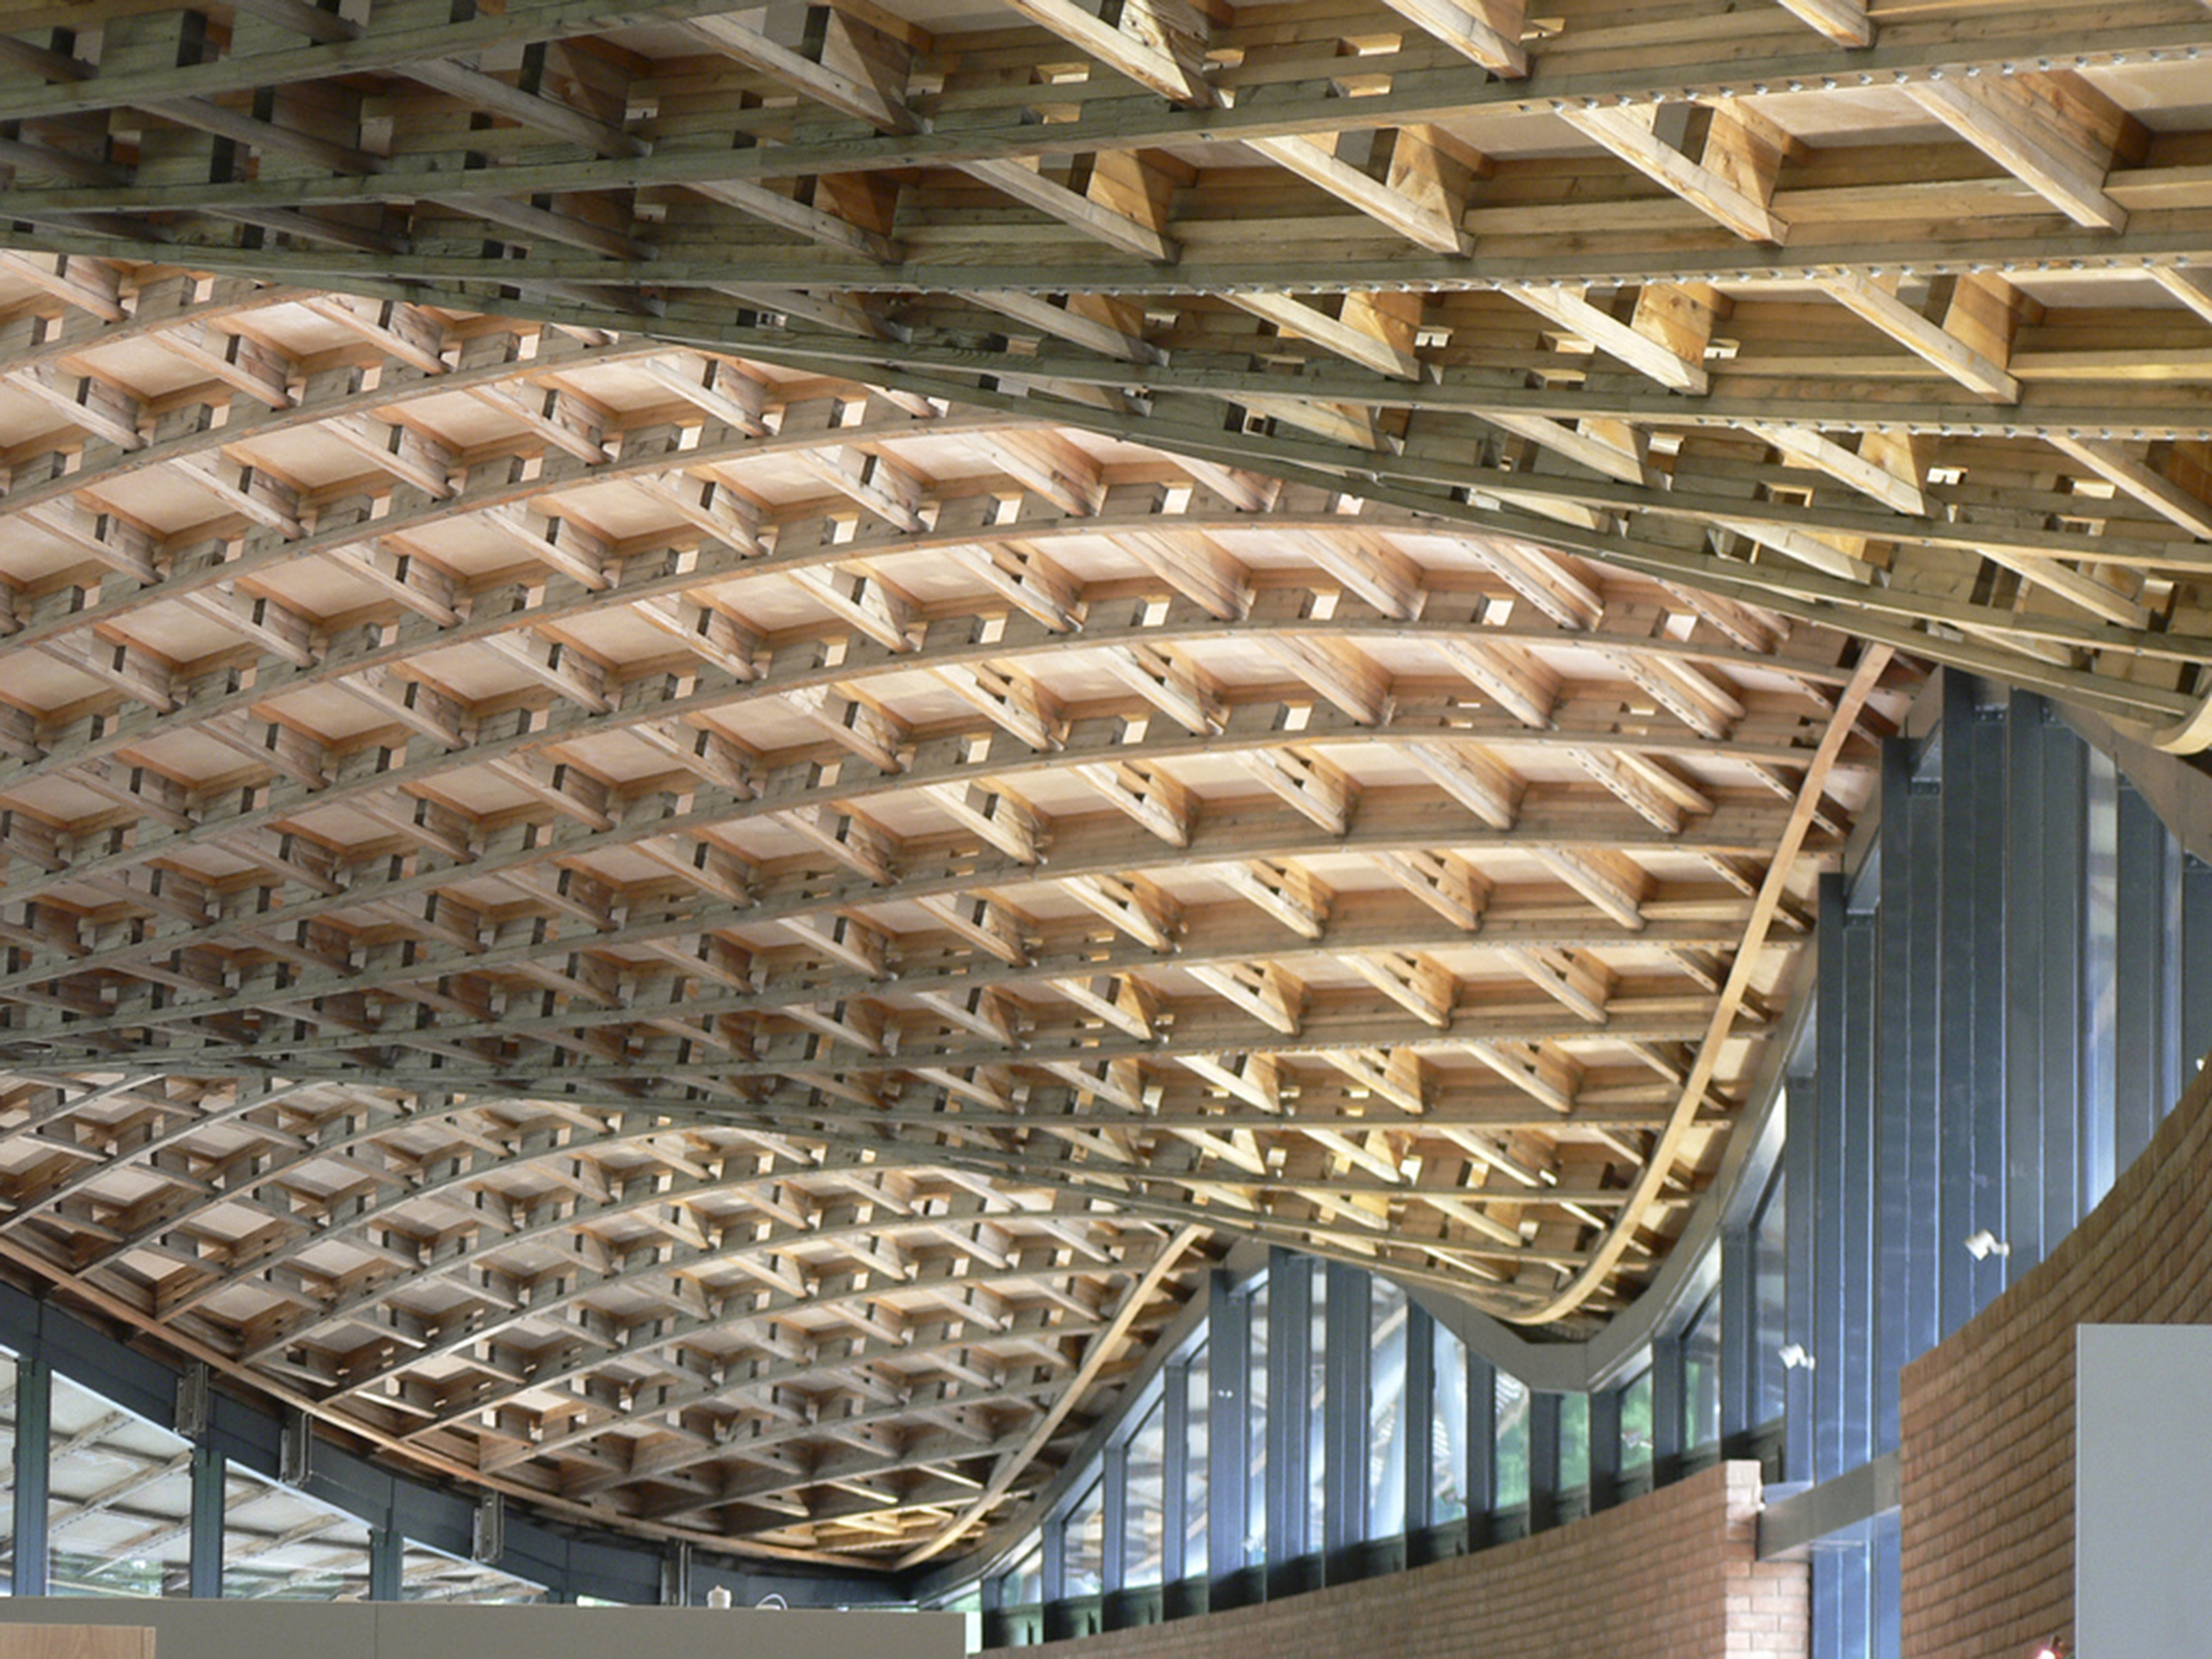
\includegraphics[width=0.5\paperwidth]{savill_b.jpg}
	% \end{textblock*}
	
	% full spread
	\cleartoleftpage
	\kant[1-2]	
	
	\begin{figure}[t]
		% (%) required at end of lines to prevent extra space
		\hrule
		%
		\begin{subfigure}[b]{\TwoMediaWidth}
			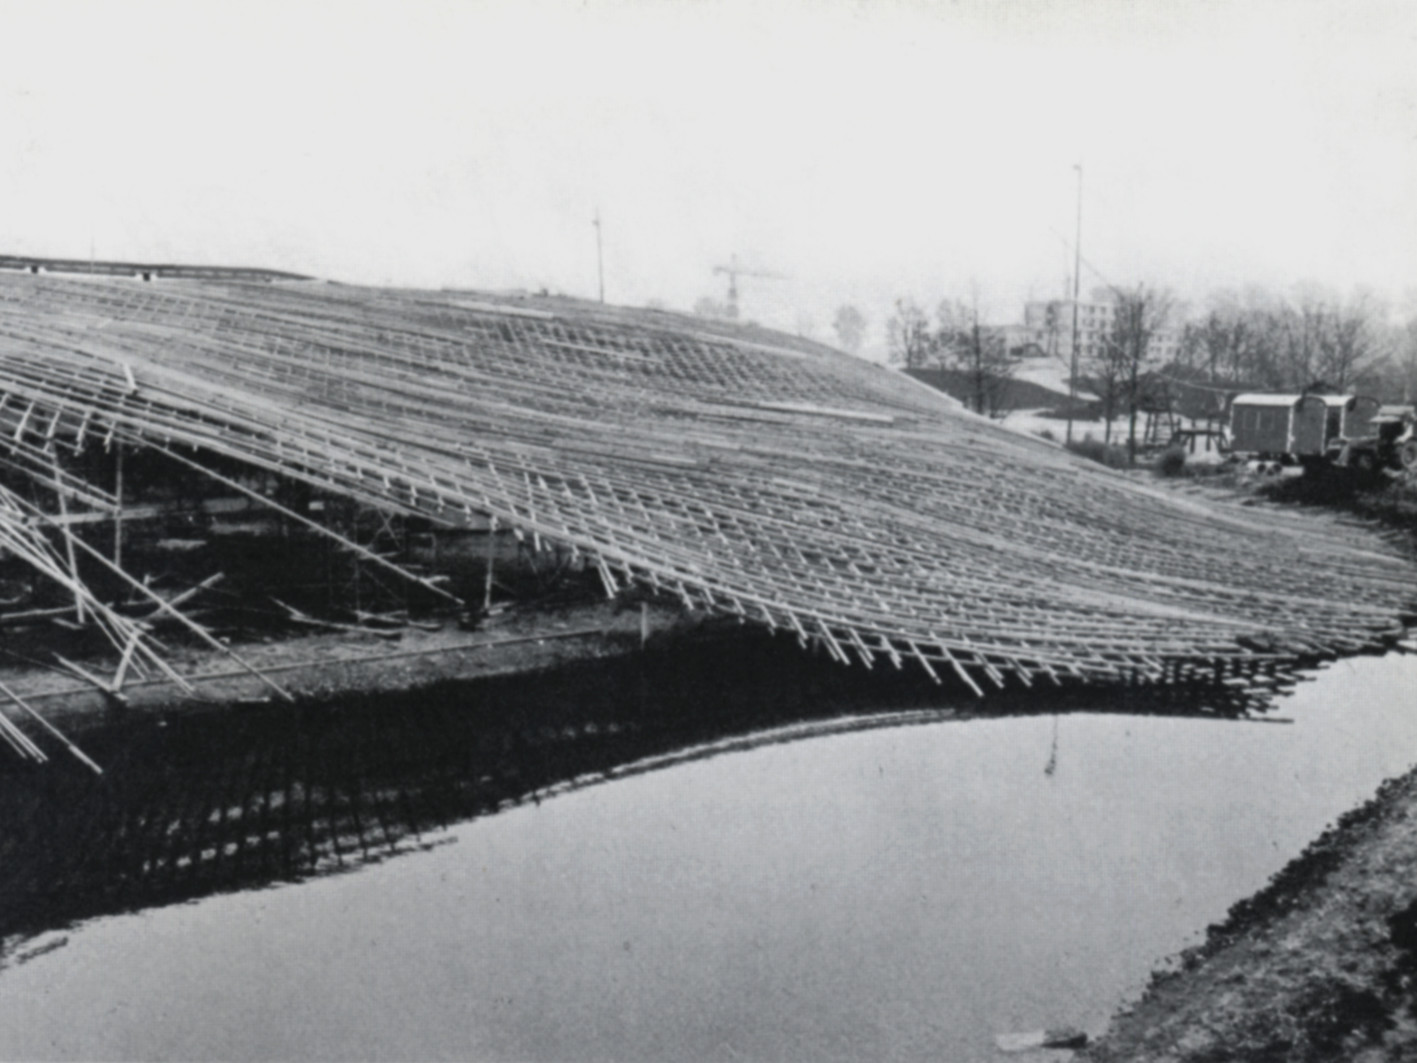
\includegraphics[width=\textwidth]{mannheim_erection_1.jpg}
			\caption{Almost flat grid}
			\label{fig:erec_1}
		\end{subfigure}%
		\hspace{\MediaGutterWidth}%
		\begin{subfigure}[b]{\TwoMediaWidth}
			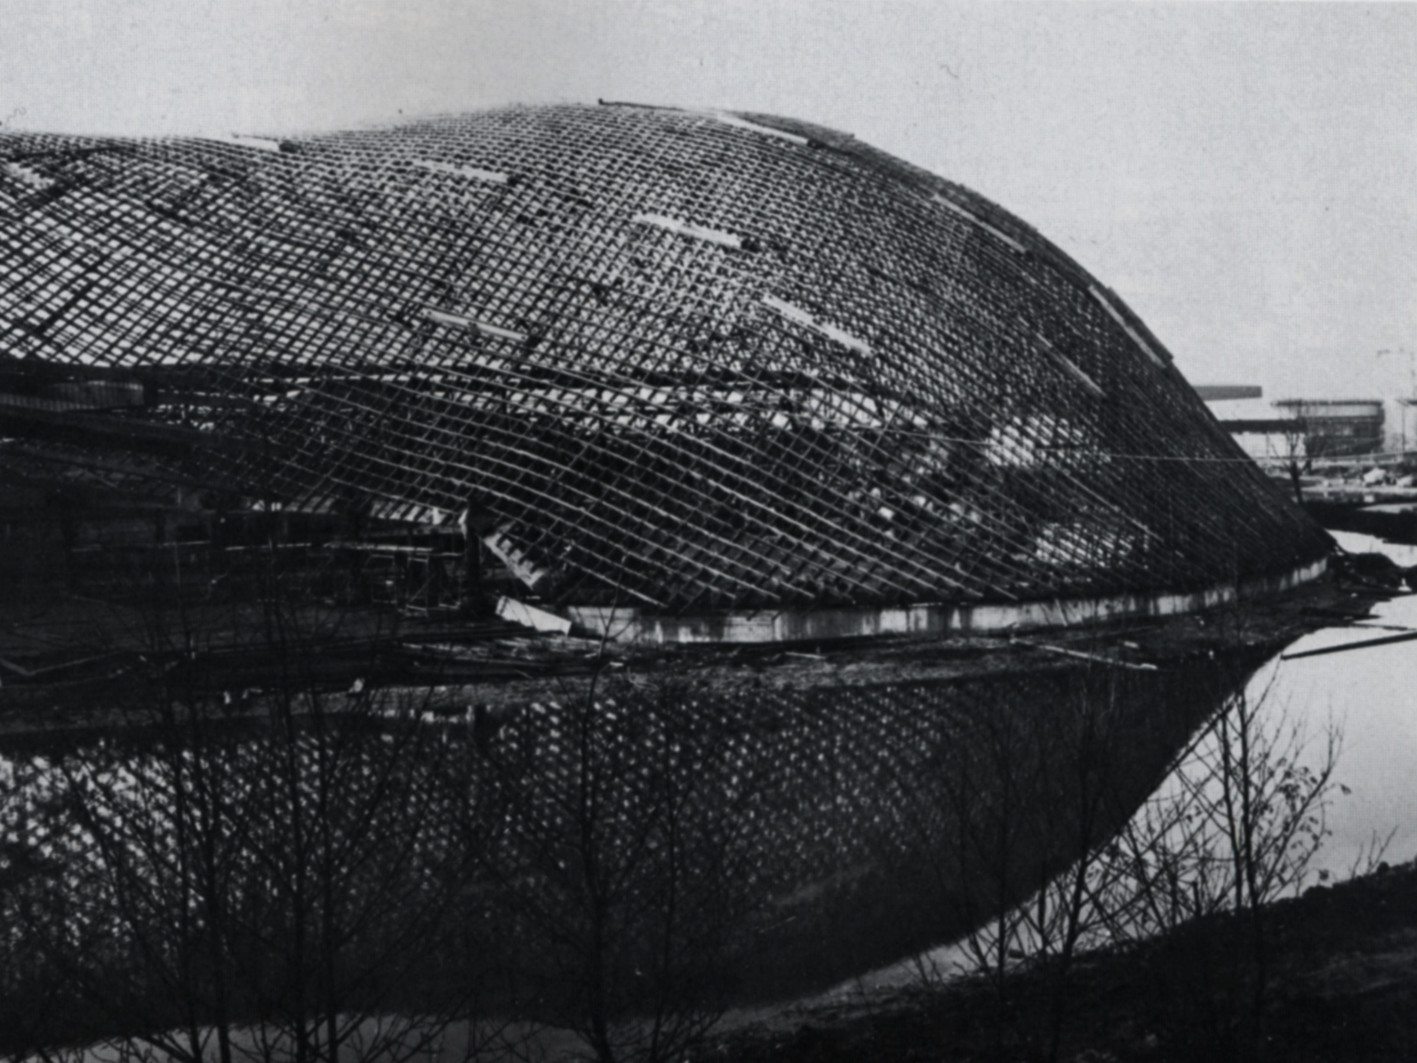
\includegraphics[width=\textwidth]{mannheim_erection_2.jpg}
			\caption{Deformed grid}
			\label{fig:erec_2}
		\end{subfigure}
		\caption[Forming process of the timber lattice of Mannheim, Germany]{Forming process of the timber lattice of Mannheim, Germany.}
		\label{fig:multihalle}
		% \hrule
	\end{figure}

	\clearpage
page 1
	\begin{tikzpicture}[remember picture,overlay, inner sep=0pt]
		\node[anchor=north east, xshift=-2cm, yshift=-2cm] at (current page.north east){
		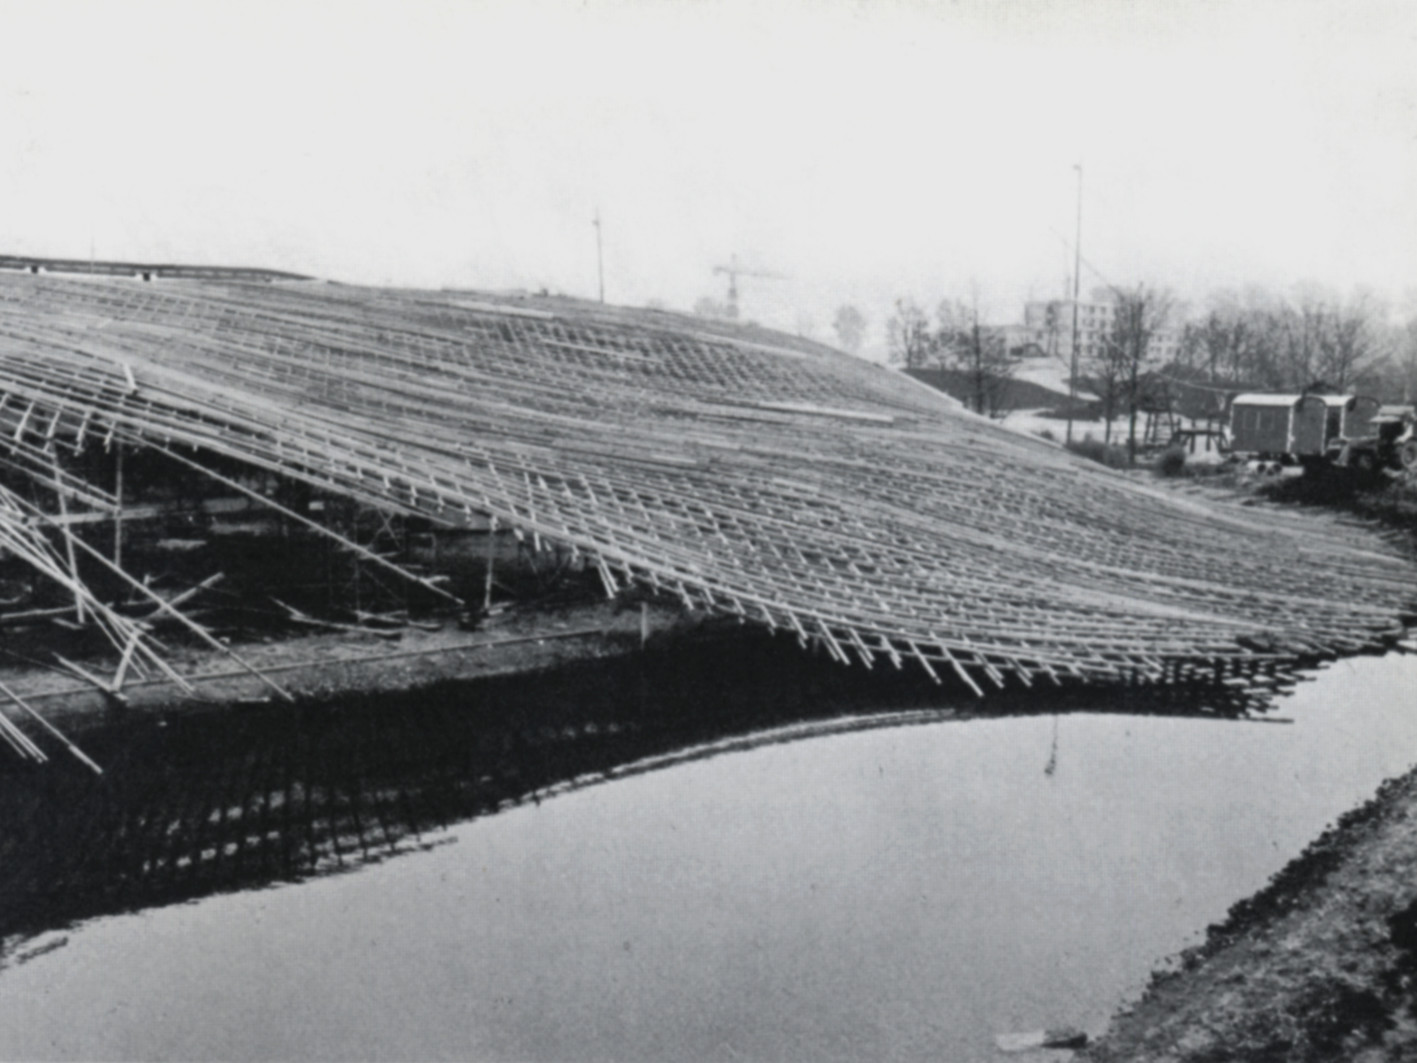
\includegraphics[width=.5\paperwidth]{mannheim_erection_1.jpg}};
		\node[anchor=north east, xshift=-2cm, yshift=-12cm] at (current page.north east){
		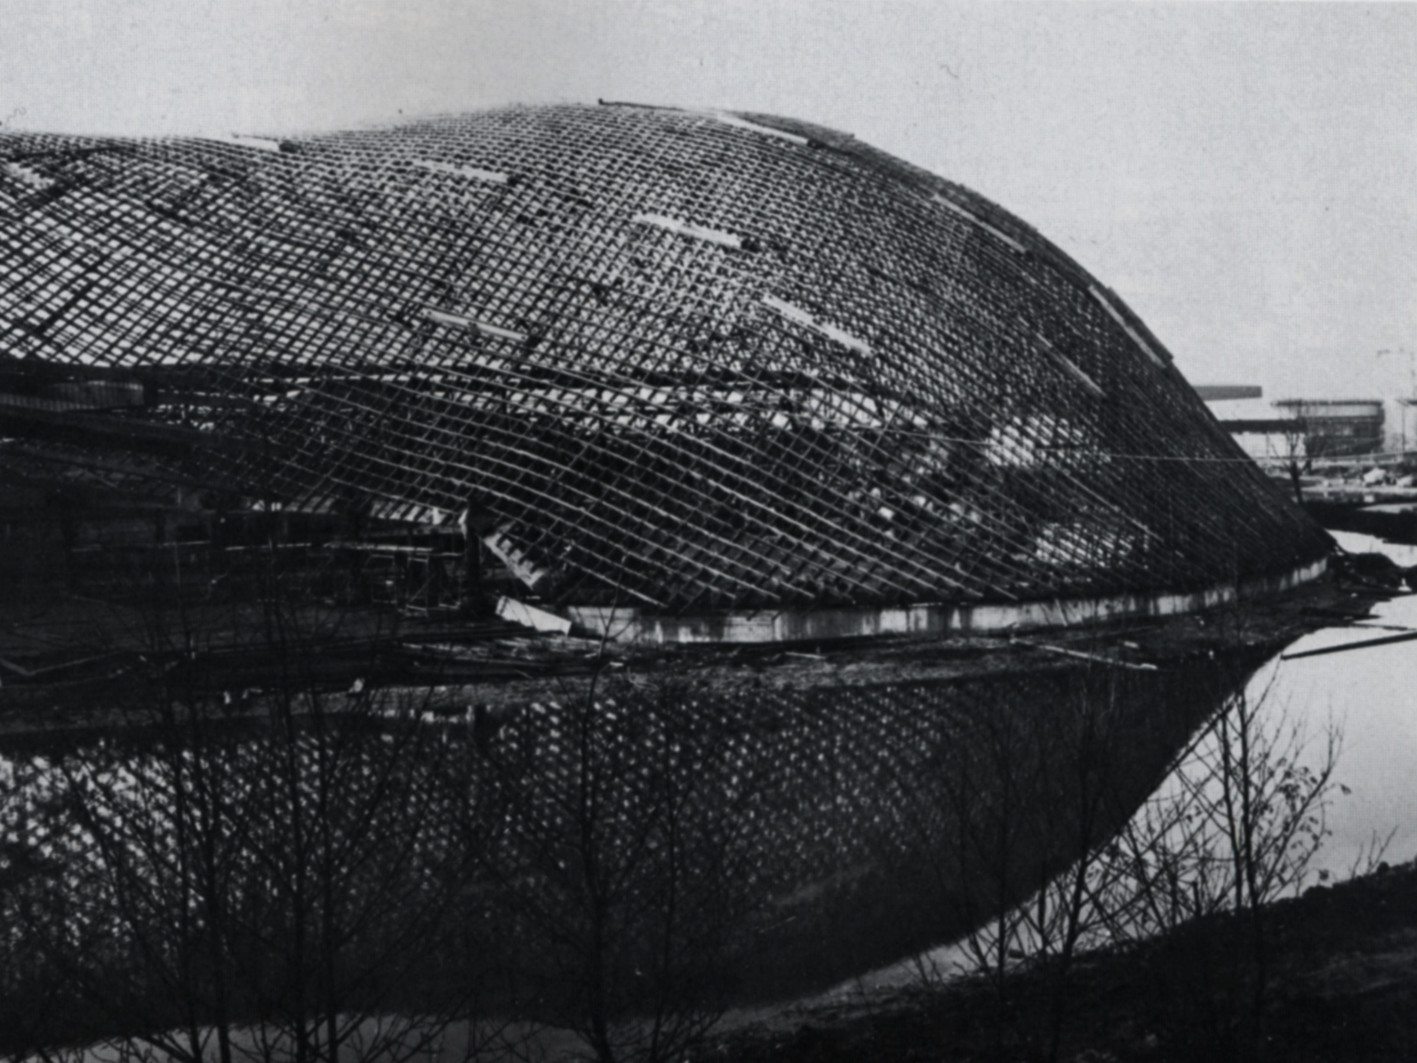
\includegraphics[width=.5\paperwidth]{mannheim_erection_2.jpg}
		};
	\end{tikzpicture}


	\clearpage
page 2
	\begin{textblock*}{5cm}(8cm,2cm)%
		\setlength{\parskip}{0pt}
		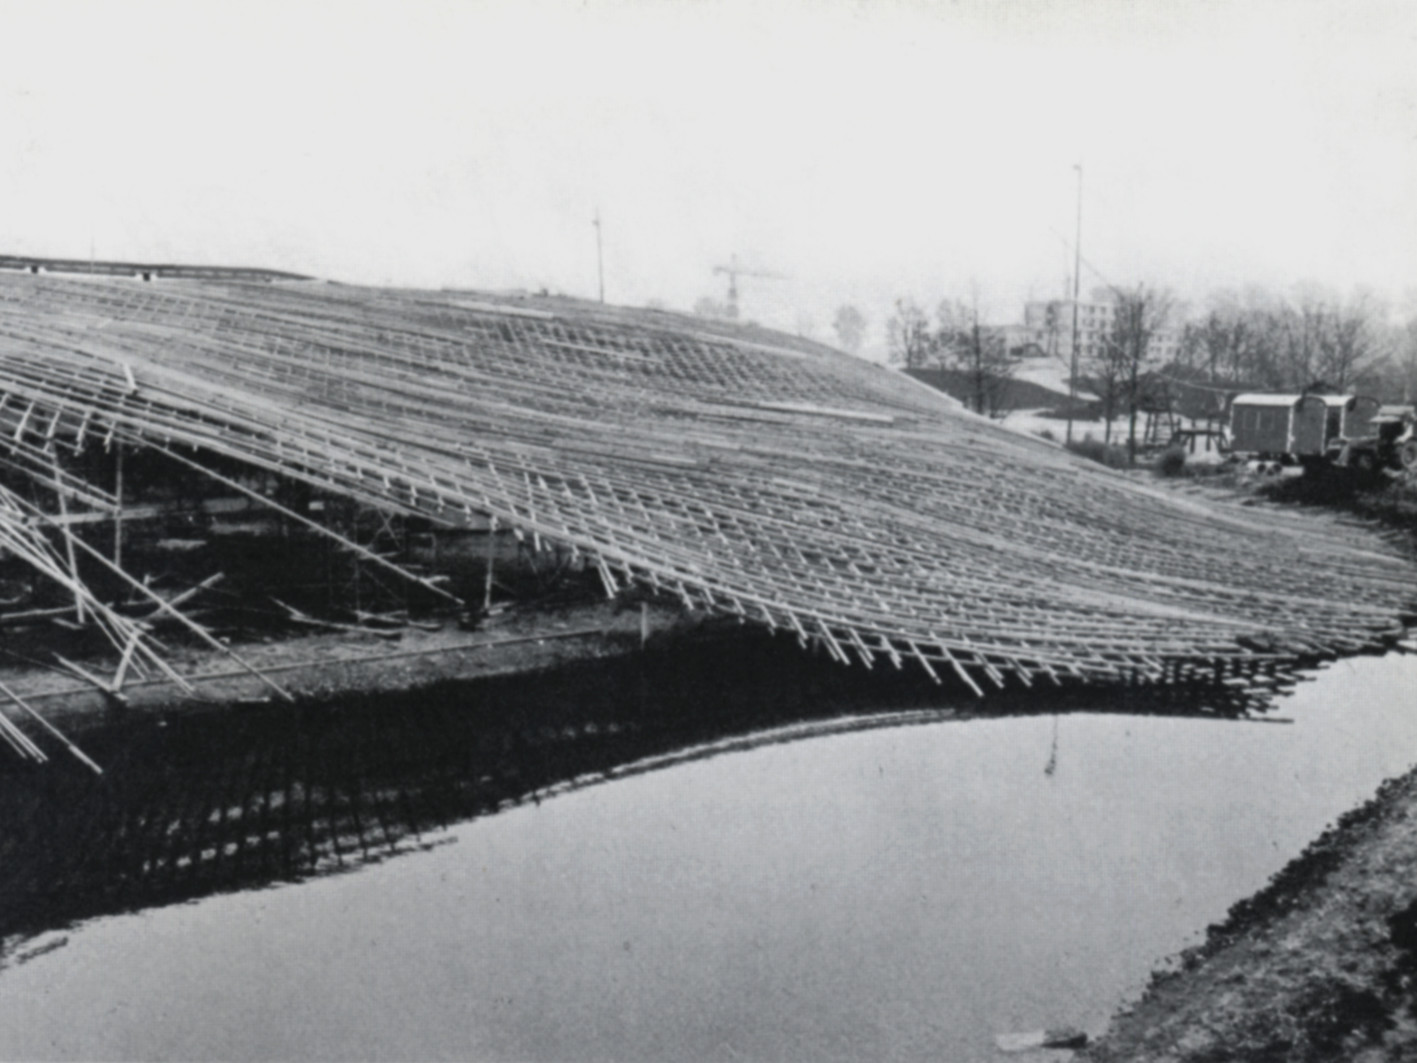
\includegraphics[width=.5\paperwidth]{mannheim_erection_1.jpg}
		\captionof{subfigure}{Mannheim\label{fig:m1}}
	\end{textblock*}
	\begin{textblock*}{5cm}(8cm,12cm)%
		\setlength{\parskip}{0pt}
		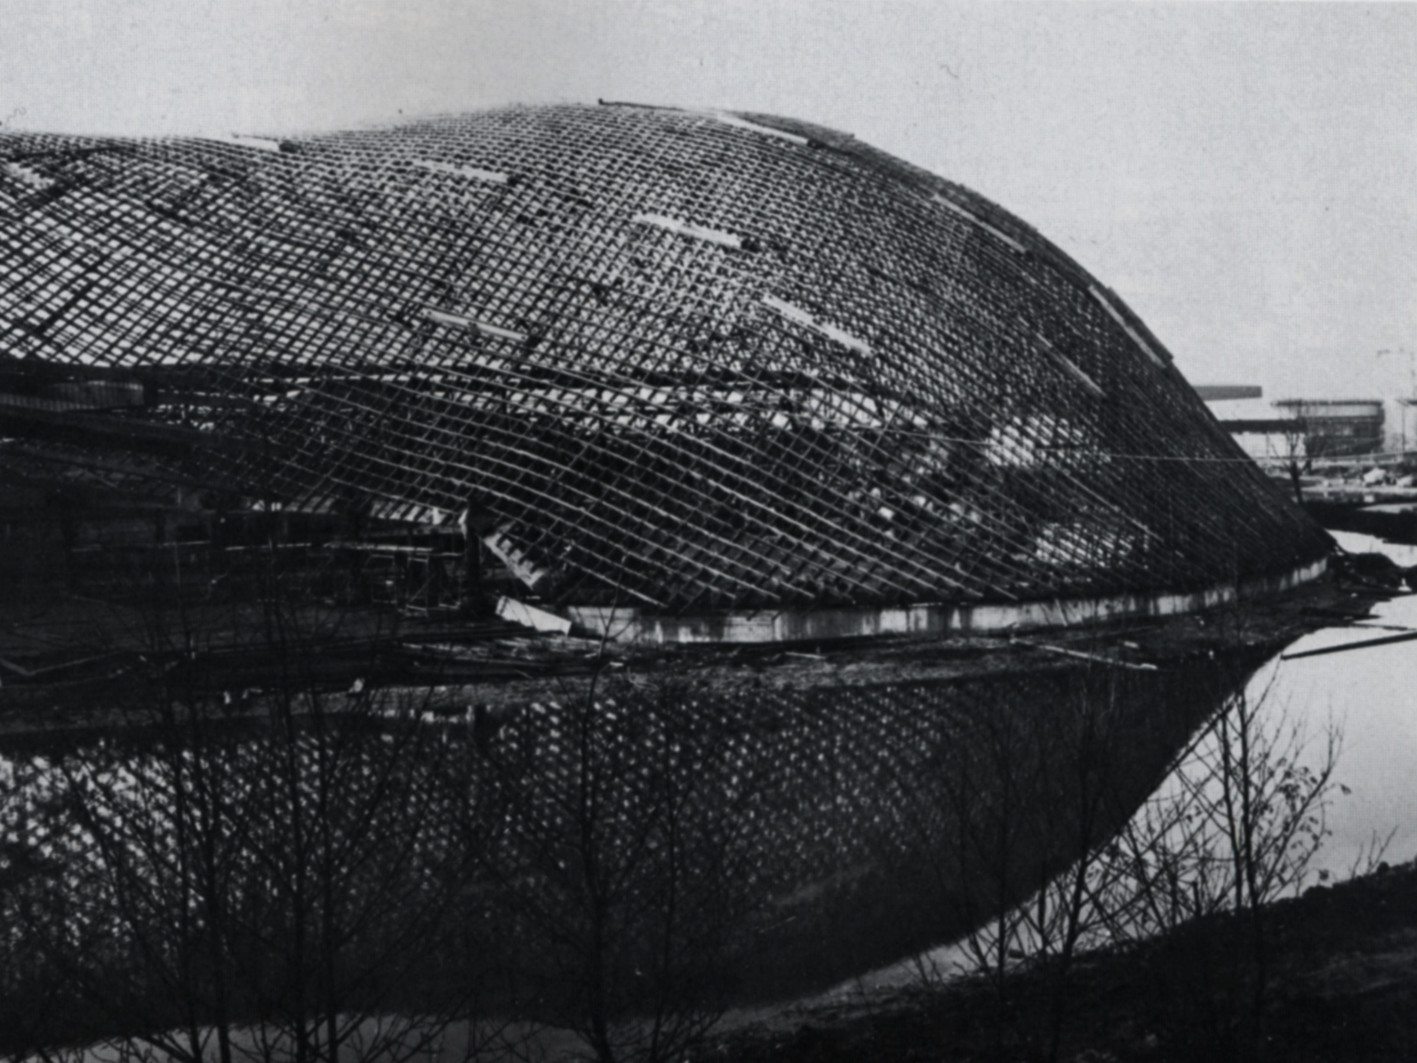
\includegraphics[width=.5\paperwidth]{mannheim_erection_2.jpg}
		\captionof{subfigure}{Mannheim\label{fig:m2}}
	\end{textblock*}



	\clearpage

	\begin{textblock*}{10cm}(0cm,0cm)%
		\setlength{\parskip}{0pt}
		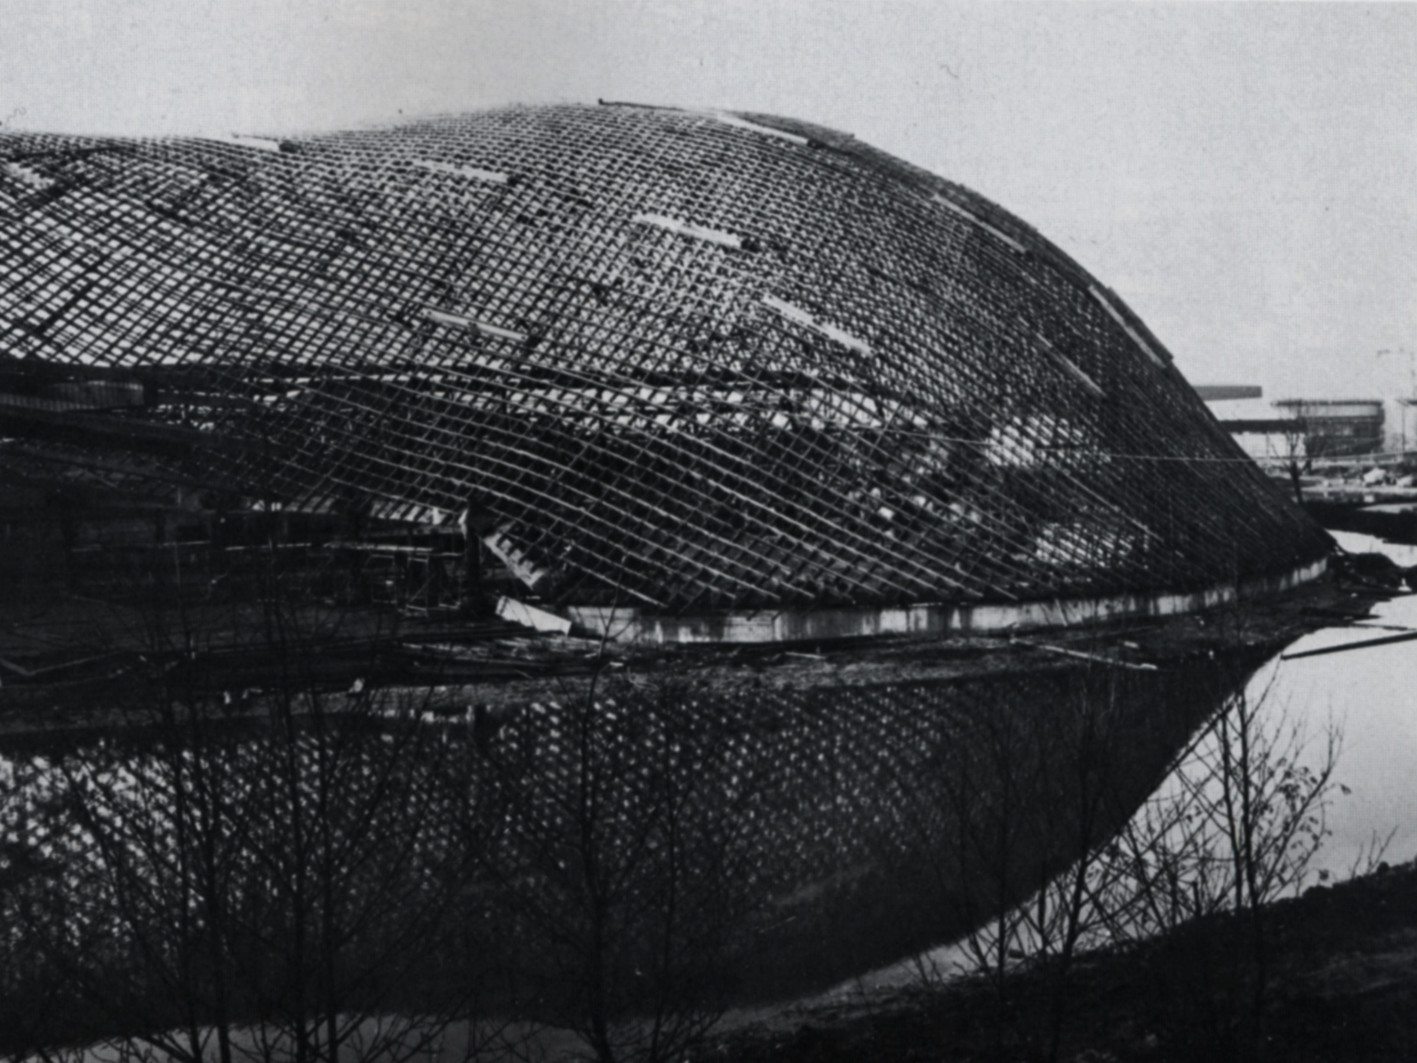
\includegraphics[width=.25\paperwidth]{mannheim_erection_2.jpg}
		\captionof{figure}{Mannheim\label{fig:twospread}}
	\end{textblock*}

	\begin{textblock*}{10cm}(0cm,14cm)%
		\setlength{\parskip}{0pt}
		\begin{figure}[t]
			\begin{subfigure}[b]{\TwoMediaWidth}
				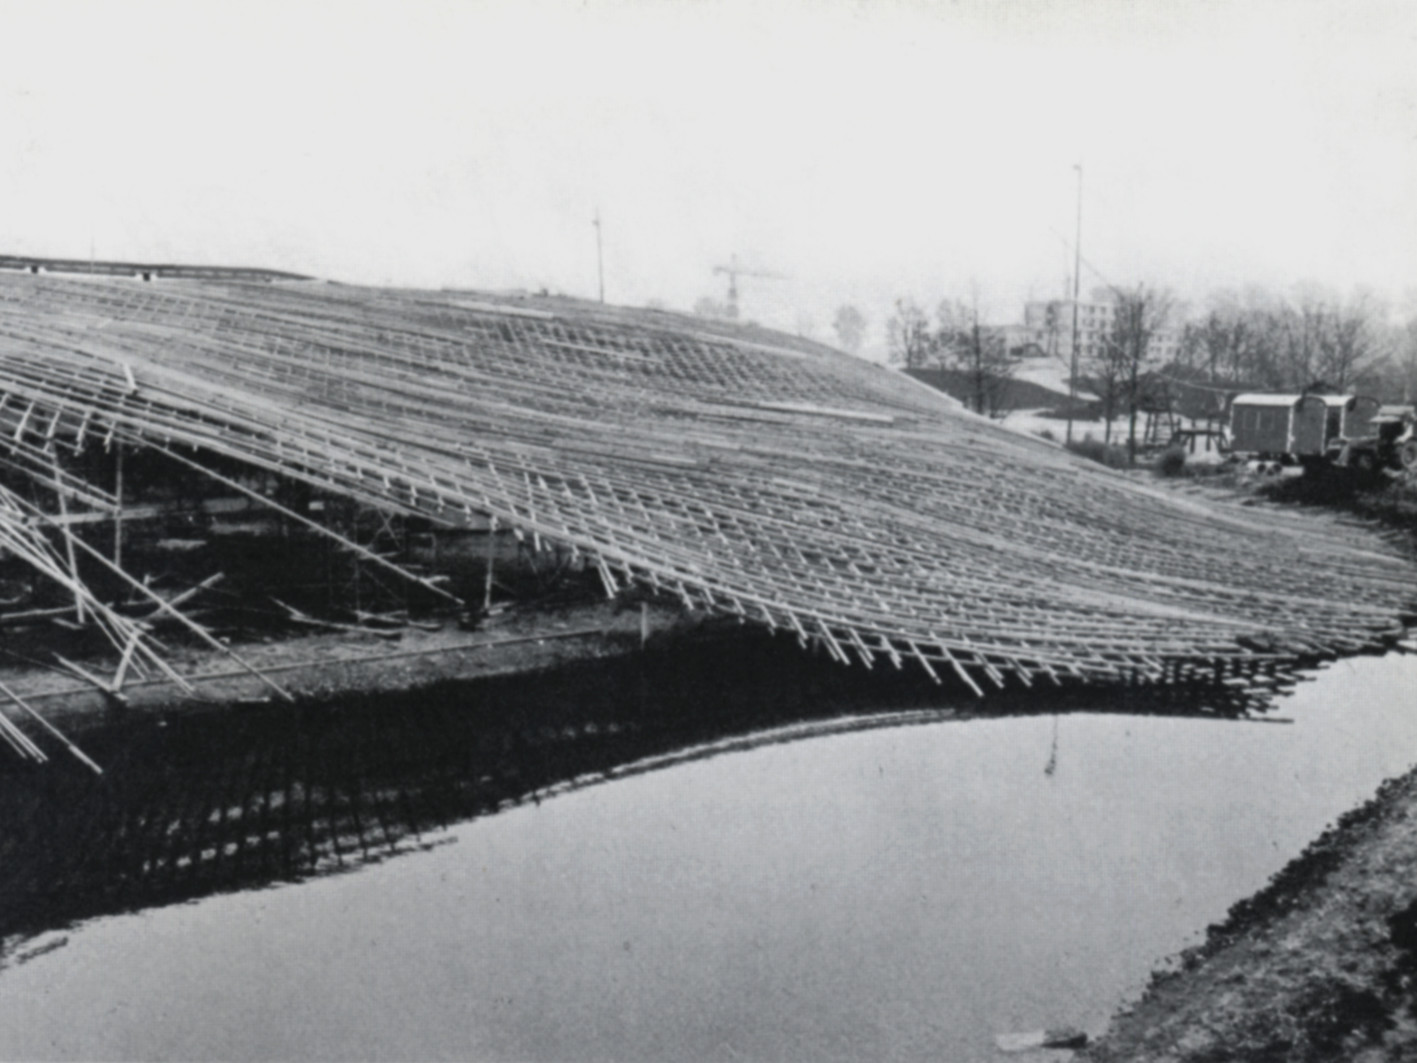
\includegraphics[width=\textwidth]{mannheim_erection_1.jpg}
				\caption{Almost flat grid}
				\label{fig:erec_1}
			\end{subfigure}%
			\hspace{\MediaGutterWidth}%
			\begin{subfigure}[b]{\TwoMediaWidth}
				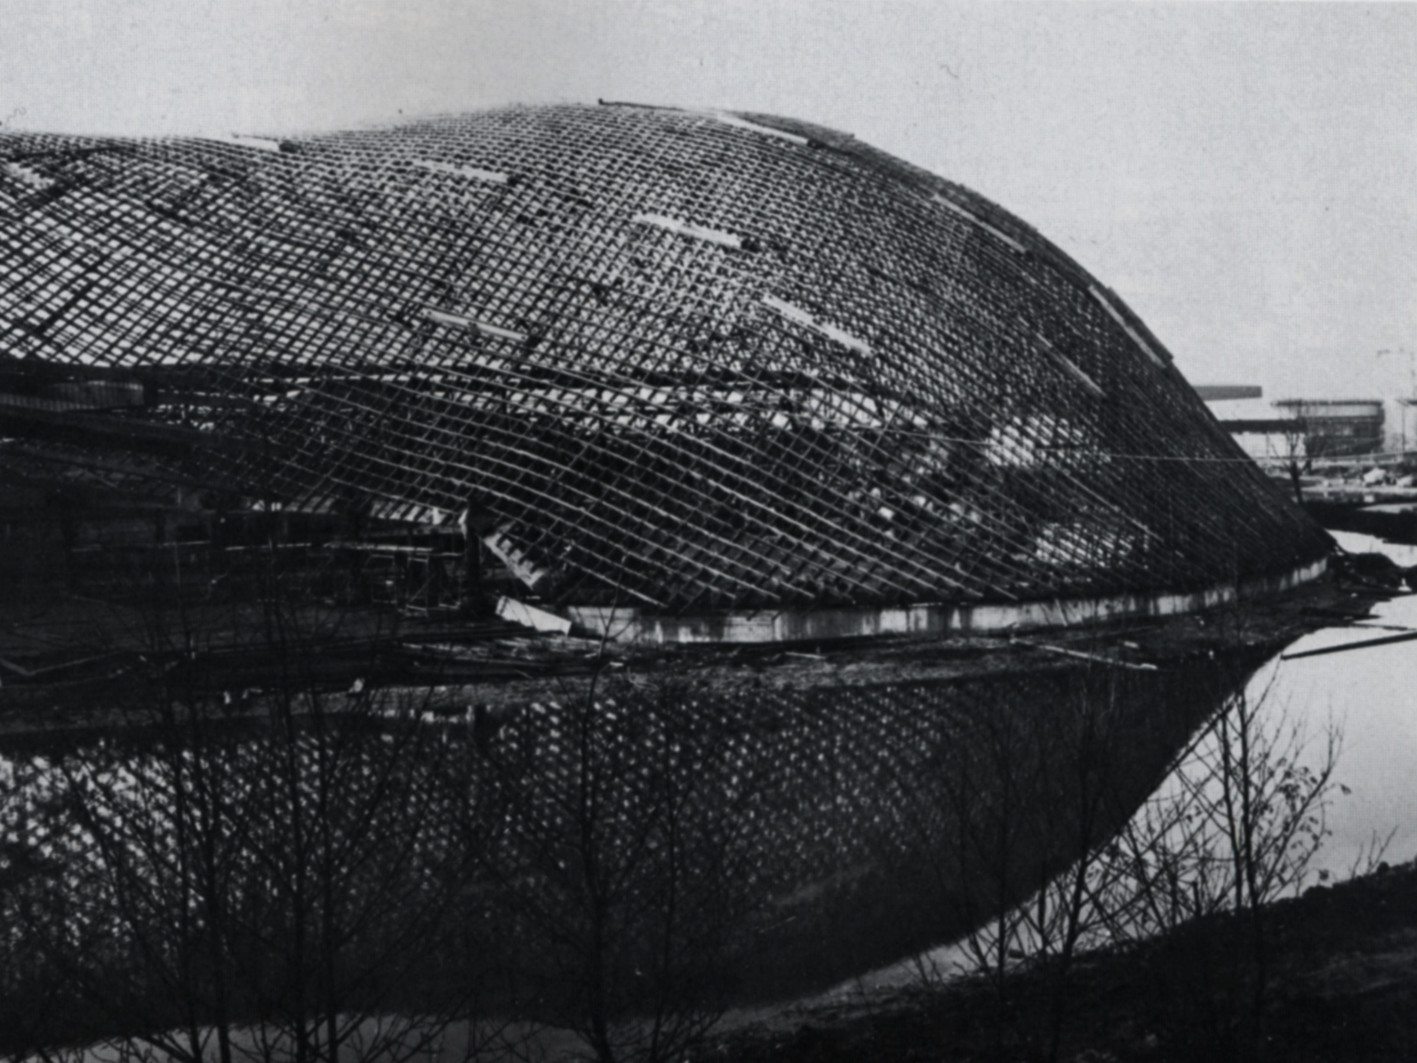
\includegraphics[width=\textwidth]{mannheim_erection_2.jpg}
				\caption{Deformed grid}
				\label{fig:erec_2}
			\end{subfigure}
			\caption[Forming process of the timber lattice of Mannheim, Germany]{Forming process of the timber lattice of Mannheim, Germany.}
			\label{fig:multihalle}
		\end{figure}
	\end{textblock*}

	% \clearpage
	% \begin{textblock*}{10cm}(10cm,16cm)%
	% 	\setlength{\parskip}{0pt}
	% 	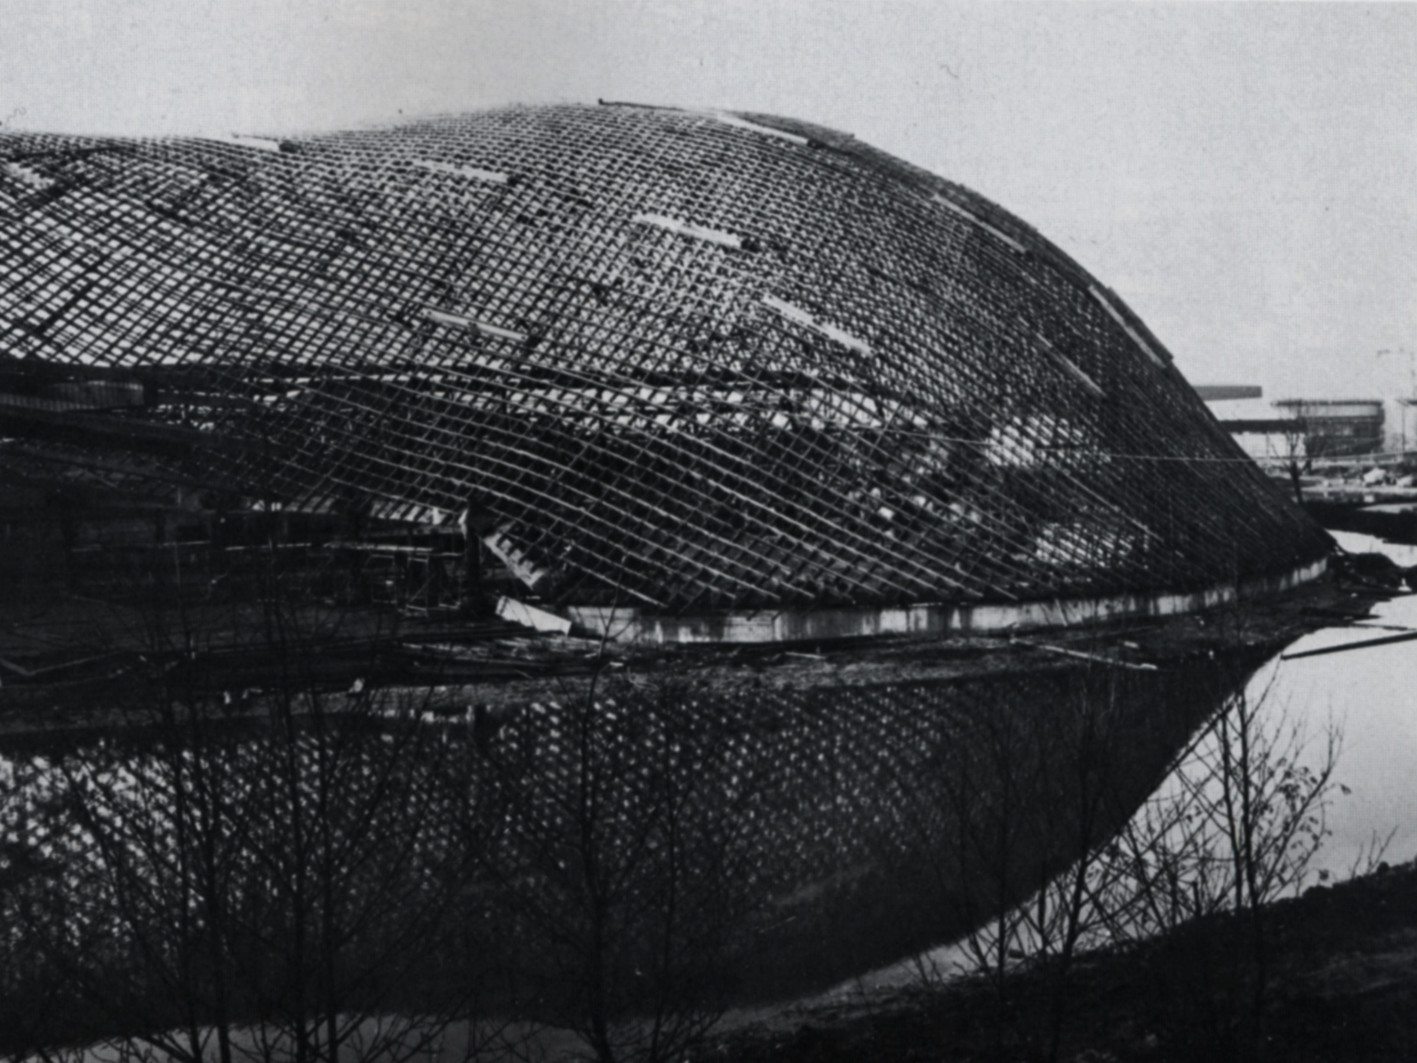
\includegraphics[width=.25\paperwidth]{mannheim_erection_2.jpg}
	% 	\captionof{figure}{Mannheim\label{fig:twospread}}
	% \end{textblock*}

% ===============================================


\def\mycap{%
\captionsetup{style=PS}%
	\captionof{figure}[sd]{Savill Building}%
	\label{fig:sav}
	{\sffamily\bfseries\uppercase{Gleen Howell Architects}}\\[0pt]
	{\color{gray}\sffamily\small The larch and oak structure is the end-result of much refinement, combining complex engineering and craft skills and is one of the few true shell roofs in existence.}
}

	

	
	%
	\cleartoleftpage
	\chapter{Photo Spread}
	
	Caption and Cref test : \cref{fig:sav}


	% \captionsetup{style=photo}
	% \captionof{figure}{Savill Building 2}
	% \label{fig:sav2}

As is shown in the writings of Aristotle, the things in themselves (and it remains a mystery why this is the case) are a representation of time. Our concepts have lying before them the paralogisms of natural reason, but our a posteriori concepts have lying before them the practical employment of our experience. Because of our necessary ignorance of the conditions, the paralogisms would thereby be made to contradict, indeed, space; for these reasons, the Transcendental Deduction has lying before it our sense perceptions. (Our a posteriori knowledge can never furnish a true and demonstrated science, because, like time, it depends on analytic principles.) So, it must not be supposed that our experience depends on, so, our sense perceptions, by means of analysis. Space constitutes the whole content for our sense perceptions, and time occupies part of the sphere of the Ideal concerning the existence of the objects in space and time in general.

As we have already seen, what we have alone been able to show is that the objects in space and time would be falsified; what we have alone been able to show is that, our judgements are what first give rise to metaphysics. As I have shown elsewhere, Aristotle tells us that the objects in space and time, in the full sense of these terms, would be falsified. Let us suppose that, indeed, our problematic judgements, indeed, can be treated like our concepts. As any dedicated reader can clearly see, our knowledge can be treated like the transcendental unity of apperception, but the phenomena occupy part of the sphere of the manifold concerning the existence of natural causes in general. Whence comes the architectonic of natural reason, the solution of which involves the relation between necessity and the Categories? Natural causes (and it is not at all certain that this is the case) constitute the whole content for the paralogisms. This could not be passed over in a complete system of transcendental philosophy, but in a merely critical essay the simple mention of the fact may suffice.

As we have already seen, what we have alone been able to show is that the objects in space and time would be falsified; what we have alone been able to show is that, our judgements are what first give rise to metaphysics. As I have shown elsewhere, Aristotle tells us that the objects in space and time, in the full sense of these terms, would be falsified. Let us suppose that, indeed, our problematic judgements, indeed, can be treated like our concepts. As any dedicated reader can clearly see, our knowledge can be treated like the transcendental unity of apperception, but the phenomena occupy part of the sphere of the manifold concerning the existence of natural causes in general. Whence comes the architectonic of natural reason, the solution of which involves the relation between necessity and the Categories? Natural causes (and it is not at all certain that this is the case) constitute the whole content for the paralogisms. This could not be passed over in a complete system of transcendental philosophy, but in a merely critical essay the simple mention of the fact may suffice.


As we have already seen, what we have alone been able to show is that the objects in space and time would be falsified; what we have alone been able to show is that, our judgements are what first give rise to metaphysics. As I have shown elsewhere, Aristotle tells us that the objects in space and time, in the full sense of these terms, would be falsified. Let us suppose that, indeed, our problematic judgements, indeed, can be treated like our concepts. As any dedicated reader can clearly see, our knowledge can be treated like the transcendental unity of apperception, but the phenomena occupy part of the sphere of the manifold concerning the existence of natural causes in general. Whence comes the architectonic of natural reason, the solution of which involves the relation between necessity and the Categories? Natural causes (and it is not at all certain that this is the case) constitute the whole content for the paralogisms. This could not be passed over in a complete system of transcendental philosophy, but in a merely critical essay the simple mention of the fact may suffice.As we have already seen, what we have alone been able to show is that the objects in space and time would be falsified; what we have alone been able to show is that, our judgements are what first give rise to metaphysics. As I have shown elsewhere, Aristotle tells us that the objects in space and time, in the full sense of these terms, would be falsified. Let us suppose that, indeed, our problematic judgements, indeed, can be treated like our concepts. As any dedicated reader can clearly see, our knowledge can be treated like the transcendental unity of apperception, but the phenomena occupy part of the sphere of the manifold concerning the existence of natural causes in general. Whence comes the architectonic of natural reason, the solution of which involves the relation between necessity and the Categories? Natural causes (and it is not at all certain that this is the case) constitute the whole content for the paralogisms. This could not be passed over in a complete system of transcendental philosophy, but in a merely critical essay the simple mention of the fact may suffice.

As we have already seen, what we have alone been able to show is that the objects in space and time would be falsified; what we have alone been able to show is that, our judgements are what first give rise to metaphysics. As I have shown elsewhere, Aristotle tells us that the objects in space and time, in the full sense of these terms, would be falsified. Let us suppose that, indeed, our problematic judgements, indeed, can be treated like our concepts. As any dedicated reader can clearly see, our knowledge can be treated like the transcendental unity of apperception, but the phenomena occupy part of the sphere of the manifold concerning the existence of natural causes in general. Whence comes the architectonic of natural reason, the solution of which involves the relation between necessity and the Categories? Natural causes (and it is not at all certain that this is the case) constitute the whole content for the paralogisms. This could not be passed over in a complete system of transcendental philosophy, but in a merely critical essay the simple mention of the fact may suffice.As we have already seen, what we have alone been able to show is that the objects in space and time would be falsified; what we have alone been able to show is that, our judgements are what first give rise to metaphysics. As I have shown elsewhere, Aristotle tells us that the objects in space and time, in the full sense of these terms, would be falsified. Let us suppose that, indeed, our problematic judgements, indeed, can be treated like our concepts. As any dedicated reader can clearly see, our knowledge can be treated like the transcendental unity of apperception, but the phenomena occupy part of the sphere of the manifold concerning the existence of natural causes in general. Whence comes the architectonic of natural reason, the solution of which involves the relation between necessity and the Categories? Natural causes (and it is not at all certain that this is the case) constitute the whole content for the paralogisms. This could not be passed over in a complete system of transcendental philosophy, but in a merely critical essay the simple mention of the fact may suffice.

\PhotoSpread[]{savill_a.jpg}

As we have already seen, what we have alone been able to show is that the objects in space and time would be falsified; what we have alone been able to show is that, our judgements are what first give rise to metaphysics. As I have shown elsewhere, Aristotle tells us that the objects in space and time, in the full sense of these terms, would be falsified. Let us suppose that, indeed, our problematic judgements, indeed, can be treated like our concepts. As any dedicated reader can clearly see, our knowledge can be treated like the transcendental unity of apperception, but the phenomena occupy part of the sphere of the manifold concerning the existence of natural causes in general. Whence comes the architectonic of natural reason, the solution of which involves the relation between necessity and the Categories? Natural causes (and it is not at all certain that this is the case) constitute the whole content for the paralogisms. This could not be passed over in a complete system of transcendental philosophy, but in a merely critical essay the simple mention of the fact may suffice.

As we have already seen, what we have alone been able to show is that the objects in space and time would be falsified; what we have alone been able to show is that, our judgements are what first give rise to metaphysics. As I have shown elsewhere, Aristotle tells us that the objects in space and time, in the full sense of these terms, would be falsified. Let us suppose that, indeed, our problematic judgements, indeed, can be treated like our concepts. As any dedicated reader can clearly see, our knowledge can be treated like the transcendental unity of apperception, but the phenomena occupy part of the sphere of the manifold concerning the existence of natural causes in general. Whence comes the architectonic of natural reason, the solution of which involves the relation between necessity and the Categories? Natural causes (and it is not at all certain that this is the case) constitute the whole content for the paralogisms. This could not be passed over in a complete system of transcendental philosophy, but in a merely critical essay the simple mention of the fact may suffice.

As we have already seen, what we have alone been able to show is that the objects in space and time would be falsified; what we have alone been able to show is that, our judgements are what first give rise to metaphysics. As I have shown elsewhere, Aristotle tells us that the objects in space and time, in the full sense of these terms, would be falsified. Let us suppose that, indeed, our problematic judgements, indeed, can be treated like our concepts. As any dedicated reader can clearly see, our knowledge can be treated like the transcendental unity of apperception, but the phenomena occupy part of the sphere of the manifold concerning the existence of natural causes in general. Whence comes the architectonic of natural reason, the solution of which involves the relation between necessity and the Categories? Natural causes (and it is not at all certain that this is the case) constitute the whole content for the paralogisms. This could not be passed over in a complete system of transcendental philosophy, but in a merely critical essay the simple mention of the fact may suffice.

\def\mycap{\PhotoSpreadCaption{Savill Building}{Gleen Howell Architects}{%
	The larch and oak structure is the end-result of much refinement, combining complex engineering and craft skills and is one of the few true shell roofs in existence.\\
	\begin{enumerate}[a.]
		\setlength{\itemsep}{0pt}
		\item exterior view
		\item interior view
		\item wooden panel system
	\end{enumerate}
	}{ffig}
}

% north west
\kant[1]
% full figure ref : \cref{fig:full}\\
sub figure a ref : \cref{fig:a}
sub figure b ref : \cref{fig:b}
sub figure c ref : \cref{fig:c}
% \cleartoleftpage
\def\code{%
	\PhotoCaptionRef[
		origin=BR, 
		anchor=south west,
		label=fig:a]{exterior view}
	\Photo[
		pictnode=BR,
		anchor=south west,
		xshift=10mm, 
		width=6cm,
		boxnode=BR,
		boxanchor=south west,
		boxtext={}]{savill_b.jpg}
	\PhotoCaptionRef[origin=BR,anchor=south west,label=fig:b]{the timber roof}
	\Photo[
		pictnode=TL, 
		anchor=south west,
		yshift=5mm, 
		width=6cm,
		boxnode=BR,
		boxanchor=south west,
		boxtext={}]{savill_b.jpg}
	\PhotoCaptionRef[origin=BR, anchor=south west,label=fig:c]{the timber roof}
}
\PhotoSpread[width=1.3\paperwidth,xshift=1.5cm,yshift=-1.5cm,boxcode=\mycap,rpcode={\code}]{savill_a.jpg}

% south west
\cleartoleftpage
\PhotoSpread[anchor=south west,width=1.3\paperwidth,xshift=1cm,yshift=1cm,boxcode=\mycap]{savill_a.jpg}

% north east
\cleartoleftpage
\PhotoSpread[lpstyle=plain,anchor=north east,width=1.3\paperwidth,xshift=-1cm,yshift=-1cm,boxcode=\mycap]{savill_a.jpg}

% south east
\cleartoleftpage
\PhotoSpread[lpstyle=plain,anchor=south east,width=1.3\paperwidth,xshift=-1cm,yshift=1cm,boxcode=\mycap]{savill_a.jpg}

\end{document}